\documentclass{beamer}

\usepackage[utf8]{inputenc}
\usepackage[T1]{fontenc}
\usepackage{textcomp}
%% Prefer Latin Modern fonts
\usepackage{lmodern}
%% Further useful packages (included in most LaTeX distributions)
\usepackage{amsmath}        % extensions for typesetting of math
\usepackage{amsfonts}       % math fonts
\usepackage{amsthm}         % theorems, definitions, etc.
\usepackage{bbding}         % various symbols (squares, asterisks, scissors, ...)
\usepackage{bm}             % boldface symbols (\bm)
\usepackage{graphicx}       % embedding of pictures
\usepackage{fancyvrb}       % improved verbatim environment
\usepackage{natbib}         % citation style AUTHOR (YEAR), or AUTHOR [NUMBER]
\usepackage{dcolumn}        % improved alignment of table columns
\usepackage{booktabs}       % improved horizontal lines in tables
\usepackage{paralist}       % improved enumerate and itemize
\usepackage{xcolor}         % typesetting in color
\usepackage{caption}
\usepackage{subcaption}
\usepackage{tikz}
\usetikzlibrary{shapes, arrows}
\usepackage{dirtytalk}
\usepackage{threeparttable}
\usepackage{fancyvrb}
\usepackage{cleveref}
\usepackage{footmisc}
\usepackage{usebib}

\definecolor{ufal}{rgb}{.956862,.482352,.1254901}
\definecolor{lightgray}{rgb}{0.93, 0.93, 0.93}
\setbeamercolor*{palette primary}{fg=ufal}
\setbeamercolor{title}{fg=ufal}
\setbeamercolor{titlelike}{fg=ufal}
\setbeamercolor{footline}{fg=gray}
% \setbeamercolor{background canvas}{bg=lightgray}
\setbeamertemplate{navigation symbols}{}
\setbeamertemplate{itemize items}[circle]
\setbeamercolor{itemize item}{fg=black}
\setbeamercolor{itemize subitem}{fg=black}
\setbeamercolor{itemize subsubitem}{fg=black}
\setbeamertemplate{footline}[frame number]

\bibinput{bibliography}

\title{Generating a Drawing According to a Textual Description}
\author{Peter Grajcar}
\date{2021}

\begin{document}

\begin{frame}[plain,noframenumbering]
    \begin{picture}(0,0)
        \put(120,40){\makebox(0,0)[rt]{
\includegraphics[height=16mm]{./figures/logo-en}}}
    \end{picture}
    \begin{center}
        \Large{\color{ufal}\inserttitle}
        \vfill
        \normalsize{\insertauthor}
        \vfill
        \small{\insertdate}
    \end{center}
\end{frame}

\begin{frame}
    \frametitle{Overview}
    \begin{itemize}
        \item Generating complex scenes with multiple objects and mutual relations between the objects.
        \item Descriptions in natural language (English).
        \item The drawing is generated from an intermediate structure -- a scene graph.
        \begin{itemize}
            \item \emph{\usebibentry{johnson2018image}{title}} by \cite{johnson2018image}.
        \end{itemize}
    \end{itemize}
    \begin{figure}[h]
    \resizebox{\textwidth}{!}{
    \begin{tikzpicture}[node distance=3cm]
     
        \draw (-80bp,75bp) node[text width=7cm]{\Large \say{A duck is swimming in a pond. A tree is next to the pond.}};
    
        \draw [->] (25bp,75bp) -- (55bp,75bp);
    
        \draw (71.0bp,46.5bp) -- (71.0bp,144.5bp) -- (274.0bp,144.5bp) -- (274.0bp,46.5bp) -- cycle;
        \draw (172.5bp,133.0bp) node {\Large group};
        \draw [->] (133.19bp,92.3bp) .. controls (152.83bp,90.652bp) and (179.94bp,88.375bp)  .. (211.85bp,85.696bp);
        \draw (172.5bp,96.0bp) node {\large IN};
        \draw [->] (133.19bp,31.497bp) .. controls (153.19bp,41.417bp) and (180.93bp,55.183bp)  .. (211.85bp,70.525bp);
        \draw (172.5bp,60.0bp) node {\large NEXT TO};
        \draw (79.0bp,76.5bp) -- (79.0bp,112.5bp) -- (133.0bp,112.5bp) -- (133.0bp,76.5bp) -- cycle;
        \draw (106.0bp,94.5bp) node {\Large duck};
        \draw (212.0bp,65.5bp) -- (212.0bp,101.5bp) -- (266.0bp,101.5bp) -- (266.0bp,65.5bp) -- cycle;
        \draw (239.0bp,83.5bp) node {\Large pond};
        \draw (79.0bp,0.5bp) -- (79.0bp,36.5bp) -- (133.0bp,36.5bp) -- (133.0bp,0.5bp) -- cycle;
        \draw (106.0bp,18.5bp) node {\Large tree};
        
        \draw [->] (285bp,75bp) -- (315bp,75bp);
        
        \draw (425bp, 75bp) node{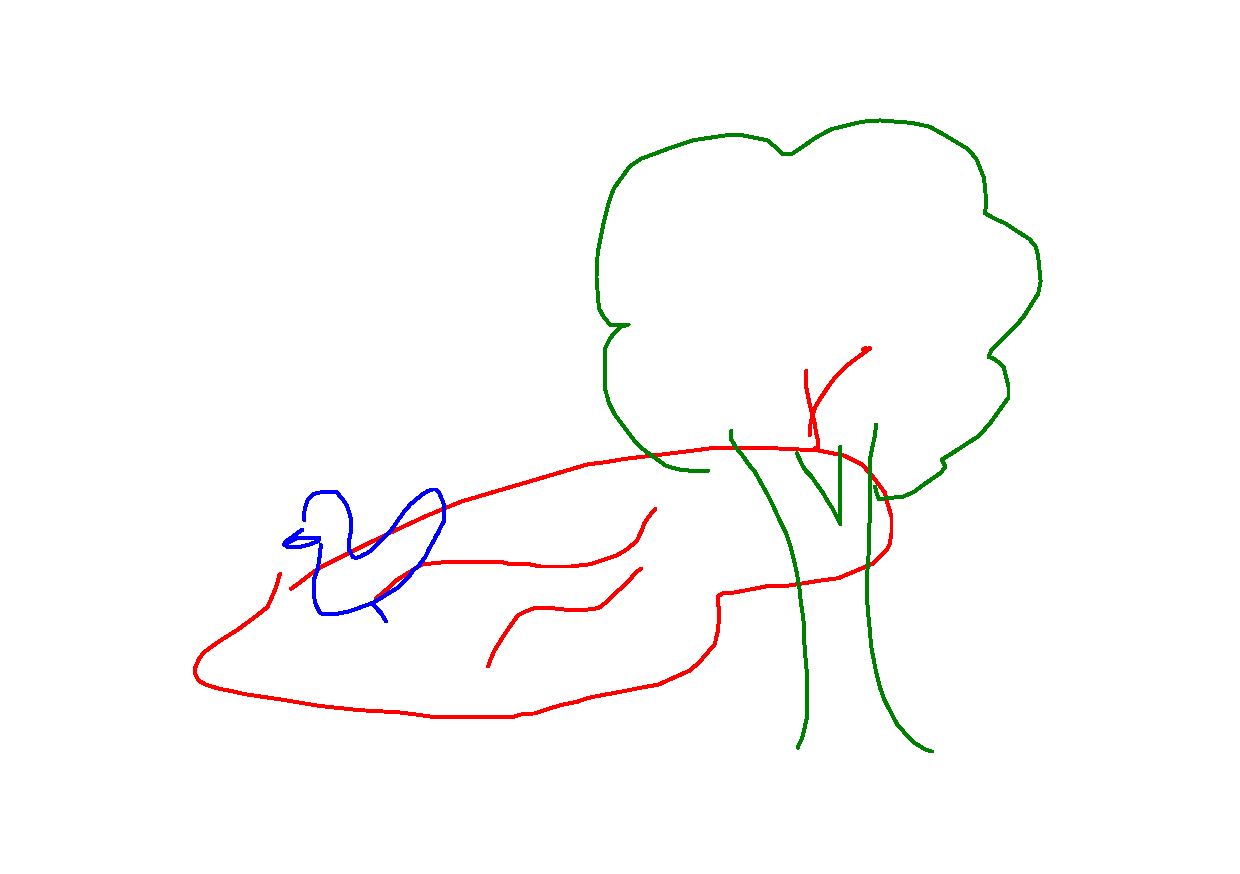
\includegraphics[width=200bp,trim=80 0 80 0,clip]{figures/duck_pond_tree_scene.pdf}};
    
    \end{tikzpicture}
    }
\end{figure}

\end{frame}

\begin{frame}
    \frametitle{Quick, Draw! Dataset}
    \begin{itemize}
        \item A crowd-sourced dataset with drawings of 345 common objects \citep{quickdraw}.
    \end{itemize}
    \begin{figure}[ht]
        \centering
        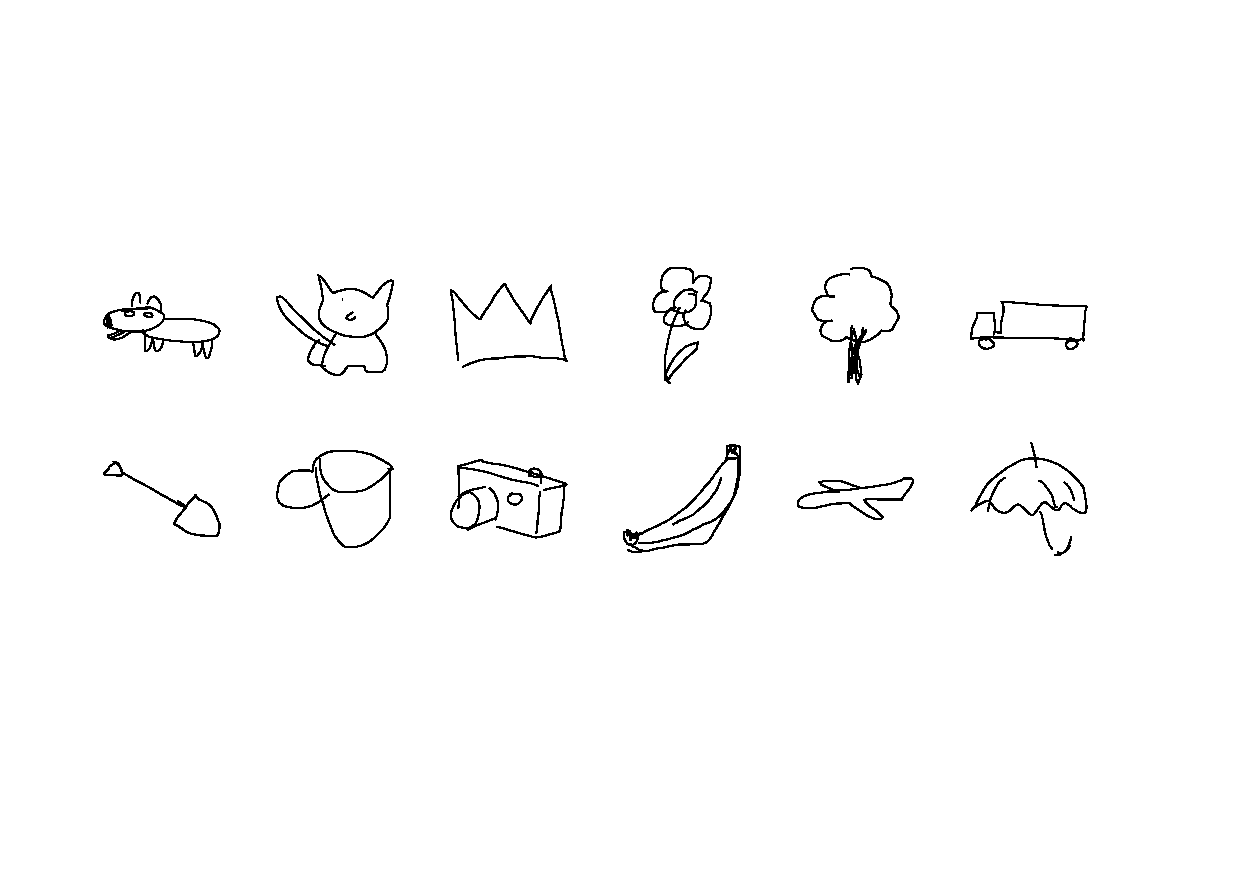
\includegraphics[width=\textwidth,trim=40 150 40 125,clip]{figures/quickdraw}
    \end{figure}
\end{frame}

\begin{frame}
    \frametitle{Scene Graphs}
    \begin{itemize}
        \item A graph-based representation of a scene.
        \item Vertices of the graph are objects and edges are relations between objects.
        \item \emph{Visual Genome} dataset \citep{krishnavisualgenome} and \emph{Scene Graph} dataset \citep{xu2017scenegraph}.
    \end{itemize}
    \begin{figure}[ht]
        \centering
        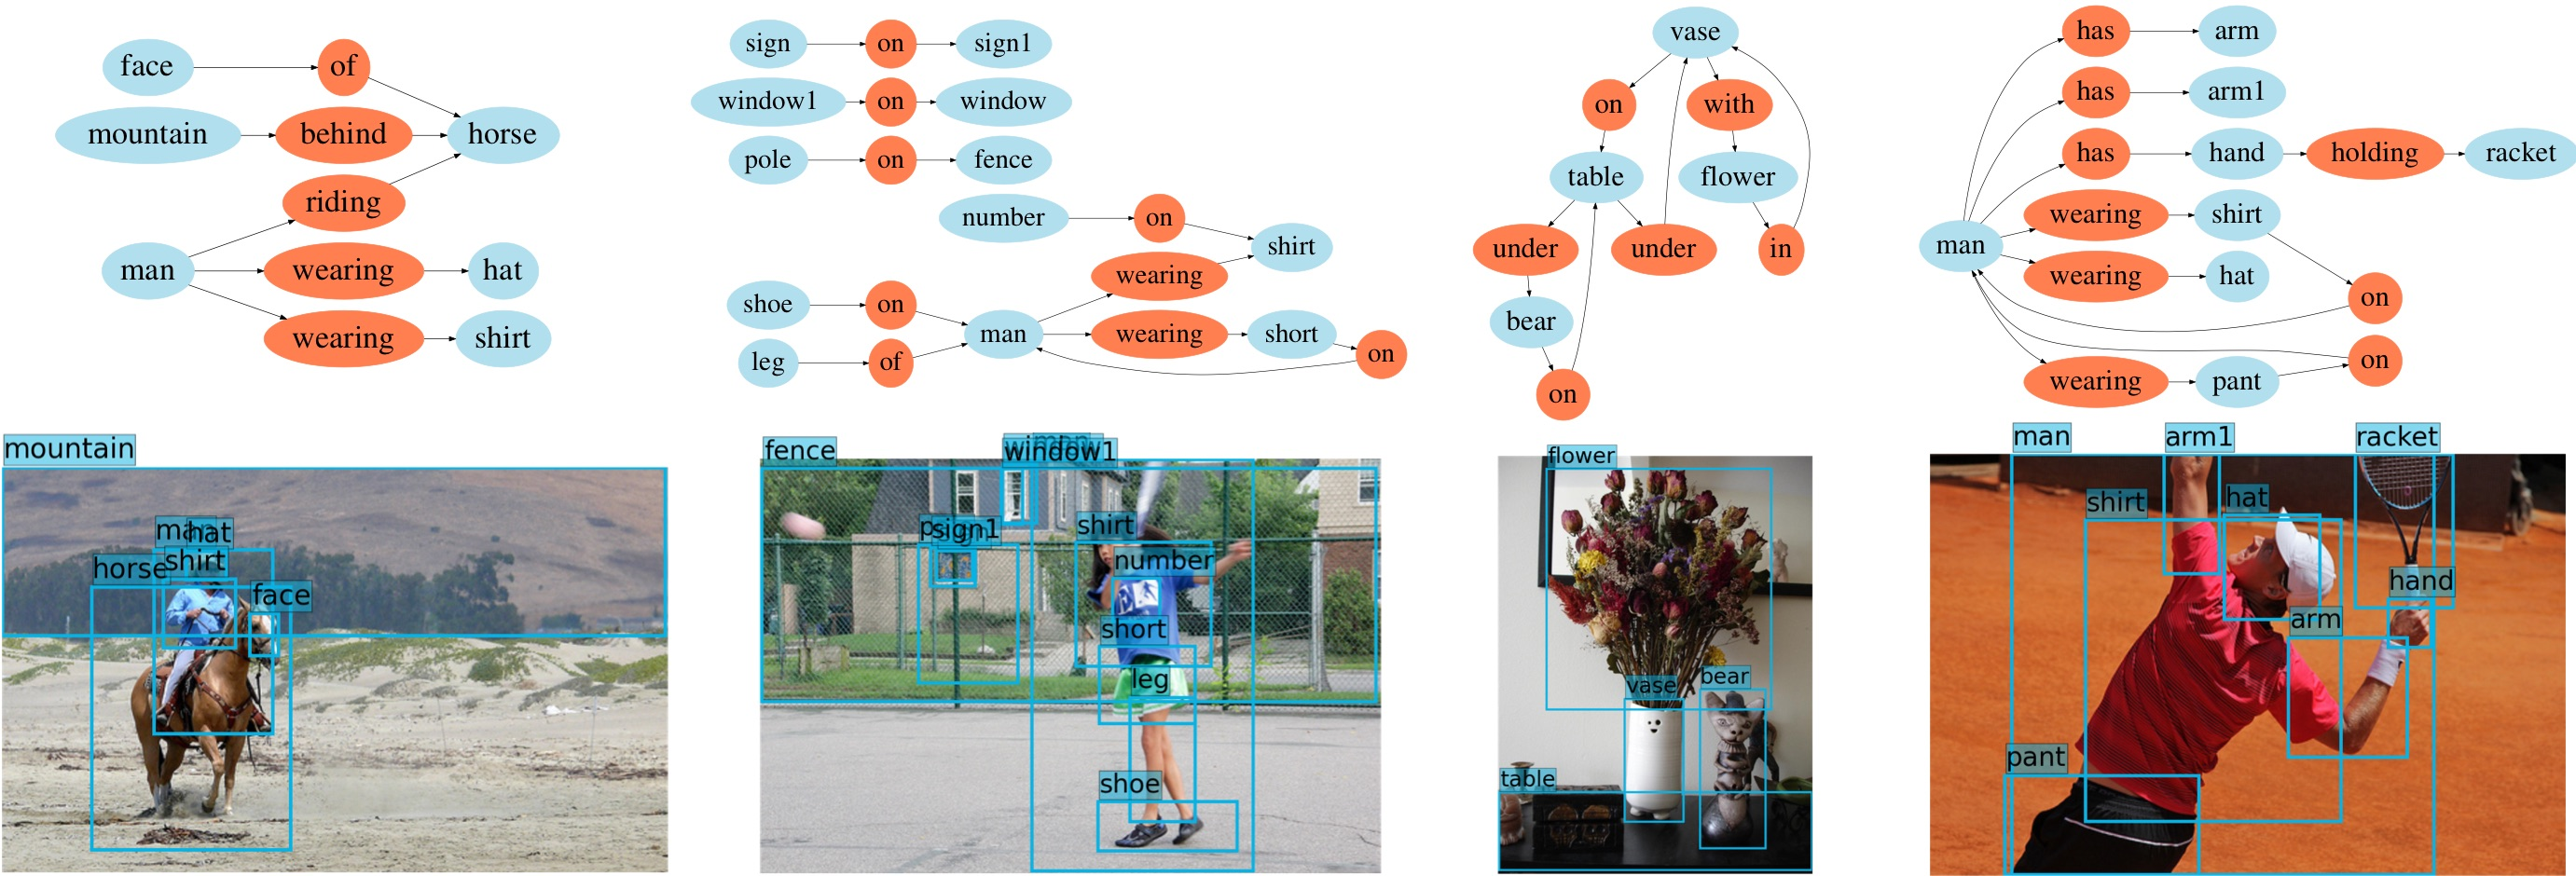
\includegraphics[width=\textwidth]{figures/scene_graph.jpeg}
        \captionsetup{font={tiny,bf,it}}
        \caption*{\hfill \color{gray}(\url{https://cs.stanford.edu/~danfei/scene-graph/})}
    \end{figure}
\end{frame}

\begin{frame}
    \frametitle{From a Description to a Scene Graph}
    \begin{itemize}
        \item Algorithm based on syntax analysis \citep{schuster2015generating}.
        \item A rule-based algorithm for object and relation retrieval.
        \begin{itemize}
            \item Interpreted as $(subject, predicate, object)$ triples.
        \end{itemize}
    \end{itemize}
    \begin{figure}
        \begin{subfigure}{0.45\textwidth}
            \centering
            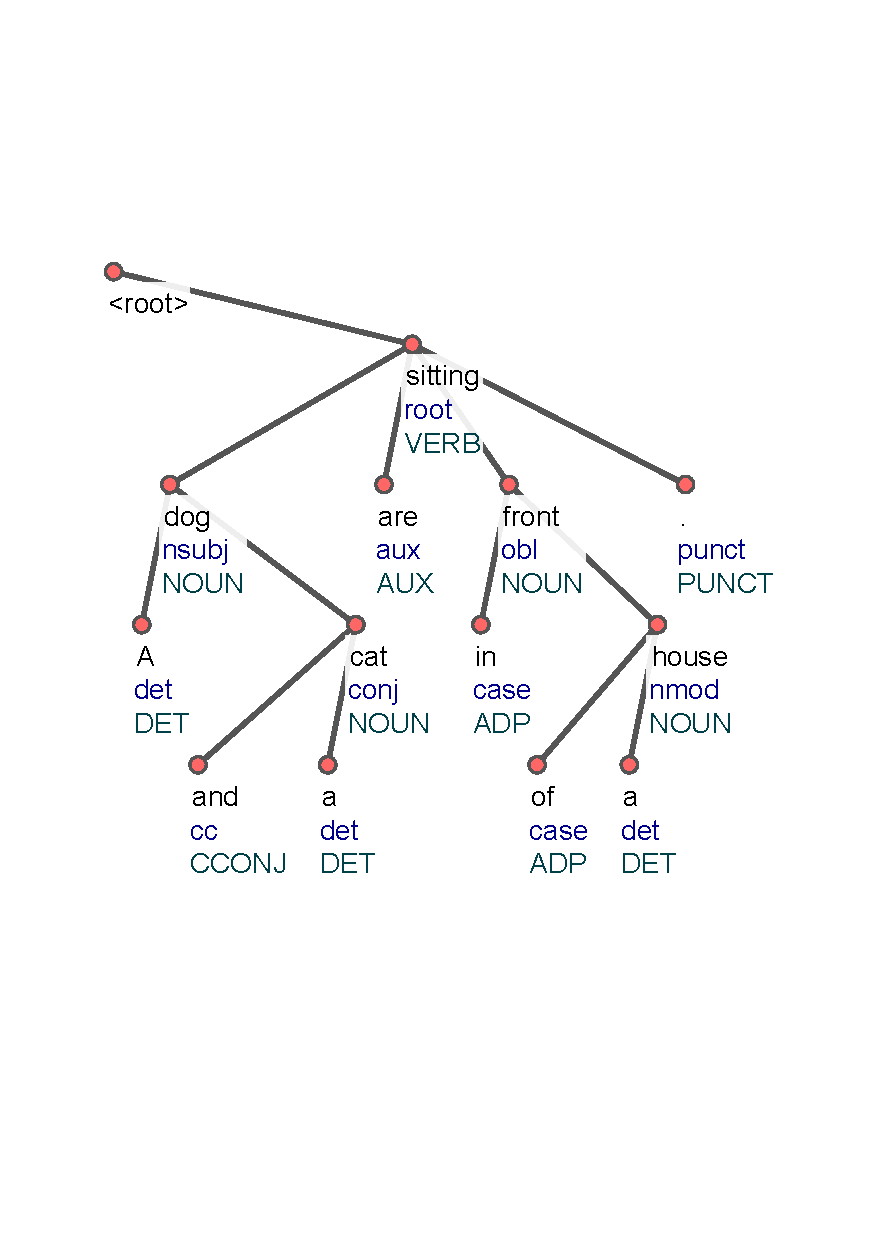
\includegraphics[width=\textwidth,trim=40 160 40 120,clip]{figures/dog_and_cat_in_front_of_house}
        \end{subfigure}
        \begin{subfigure}{0.45\textwidth}
            \centering
            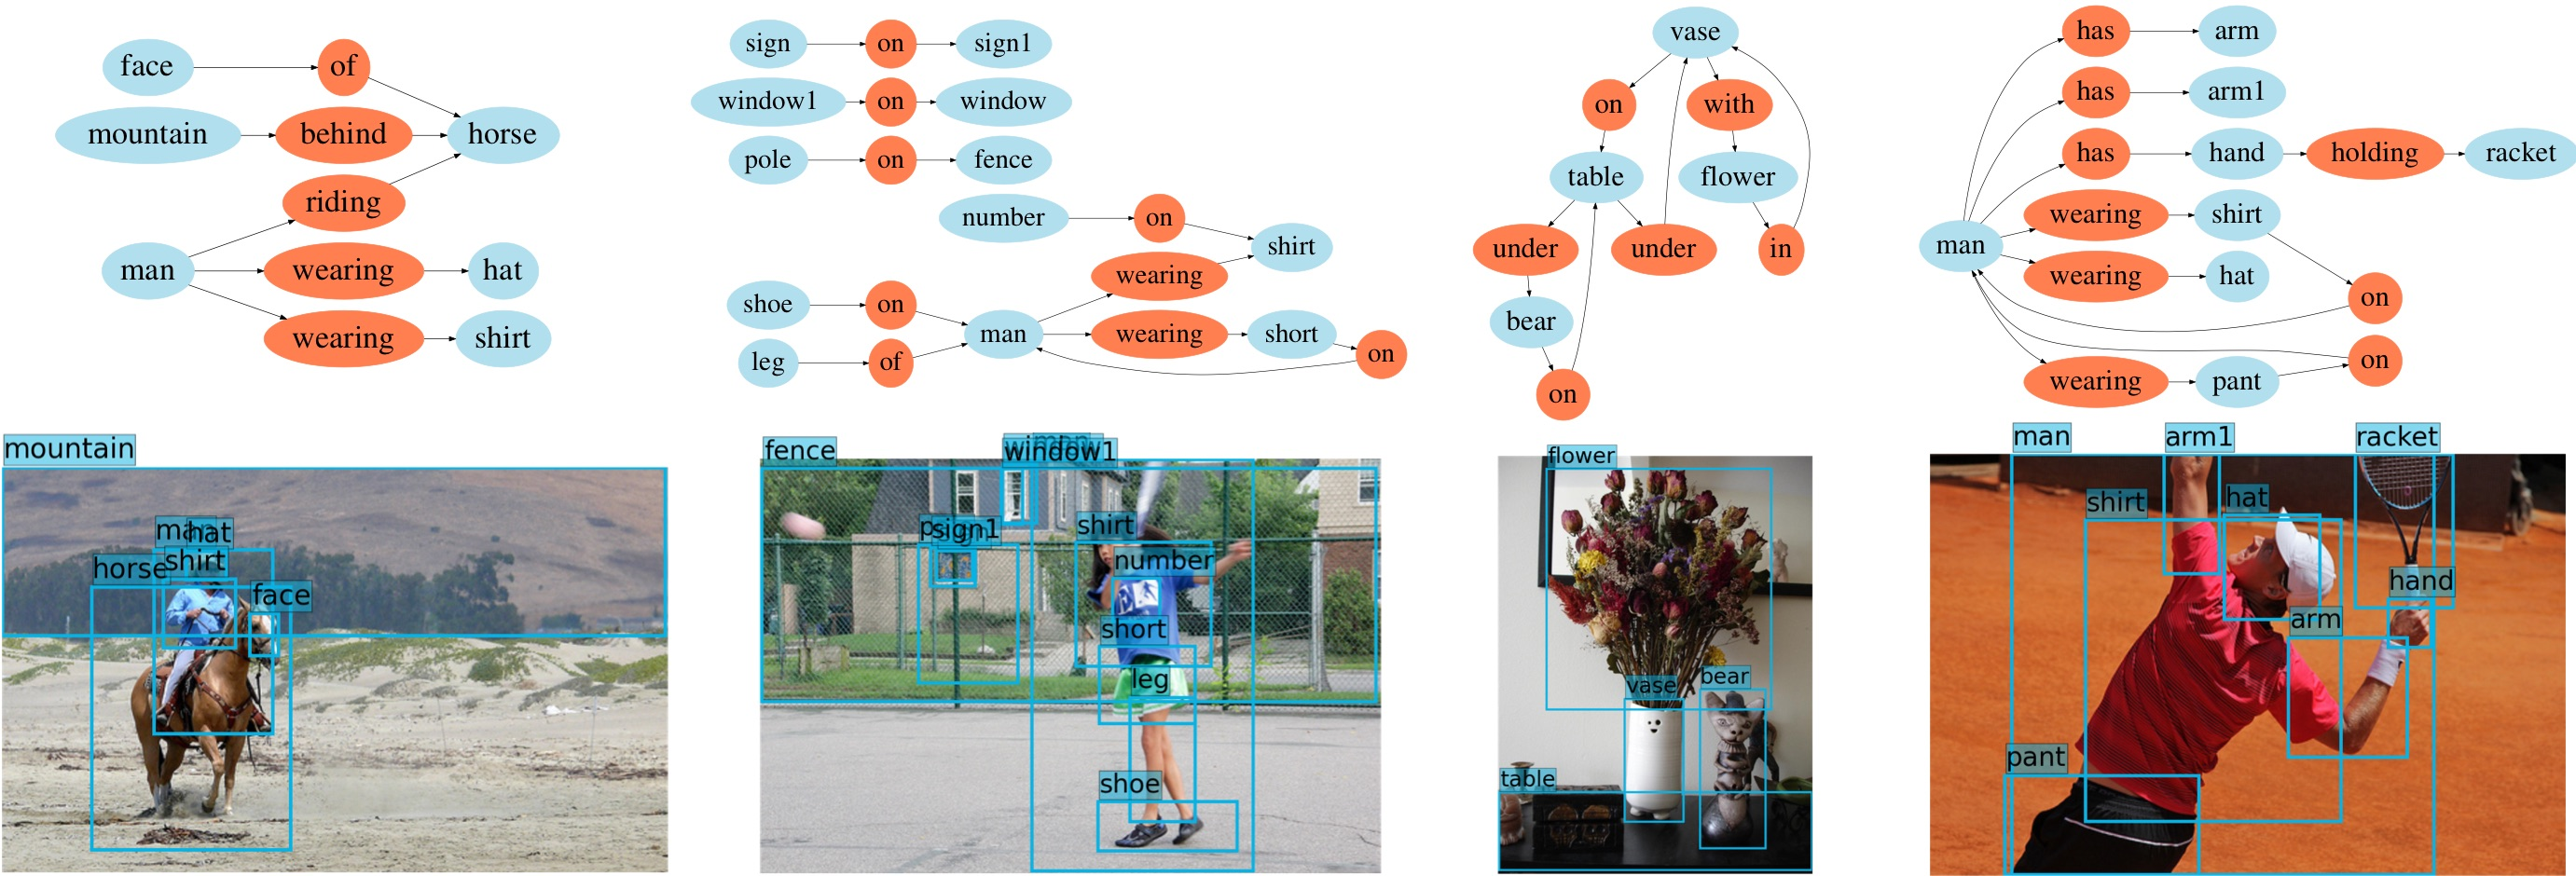
\includegraphics[width=\textwidth,trim=40 40 40 40,clip]{figures/scene_graph}
        \end{subfigure}
        \captionsetup{font={tiny,bf,it},justification=raggedright,singlelinecheck=false}
        \caption*{\color{gray}(\url{https://lindat.mff.cuni.cz/services/udpipe/})}
    \end{figure}
\end{frame}

\begin{frame}
    \frametitle{Determining Object's Position}
    \begin{itemize}
        \item Methods used in related work:
        \begin{itemize}
            \item \cite{johnson2018image} used box regression -- predicting the bounding box of the object.
            \item \cite{tripathi2019using} improved the original box regression method proposed by
                \cite{johnson2018image}.
        \end{itemize}
        \item We introduce a constraint function for every $(a, p, b)$ semantic subject, predicate, object triple.
        \begin{align*}
            C_{a,b}^p\colon \mathbb{R}^2 \rightarrow \{0, 1\}
        \end{align*}
        \item Defining the constraint function:
        \begin{itemize}
            \item A rule based approach.
            \item A classifier based approach.
        \end{itemize}
    \end{itemize}
\end{frame}
\begin{frame}
    \frametitle{Determining Object's Position}
    \begin{itemize}
        \item To determine the position of a given object $a$ we need to find a point $(x, y) \in \mathbb{R}^2$ such
        that $C_{a,b_i}^{p_i}(x, y) = 1$ for every $(a, p_i, b_i)$.
        \begin{itemize}
            \item Hard to make any assumptions about the constraint function.
            \item Monte Carlo method:
        \end{itemize}
    \end{itemize}
    \begin{figure}[ht]
        \centering
        \begin{subfigure}{0.45\textwidth}
            \centering
            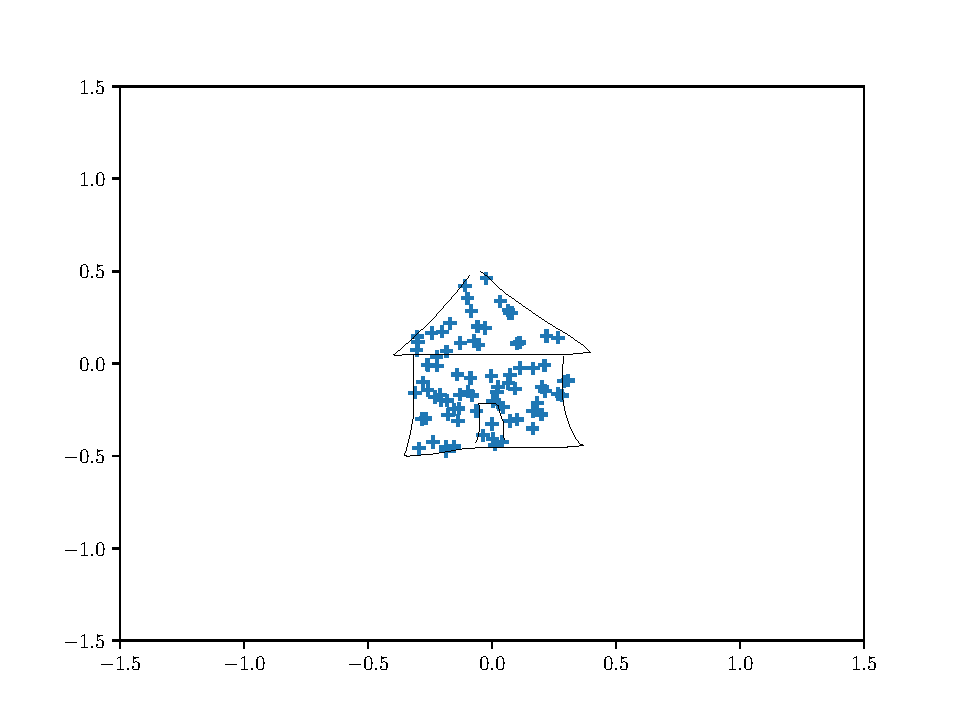
\includegraphics[width=\textwidth]{figures/rule_in_house.pdf}
        \end{subfigure}
        \begin{subfigure}{0.45\textwidth}
            \centering
            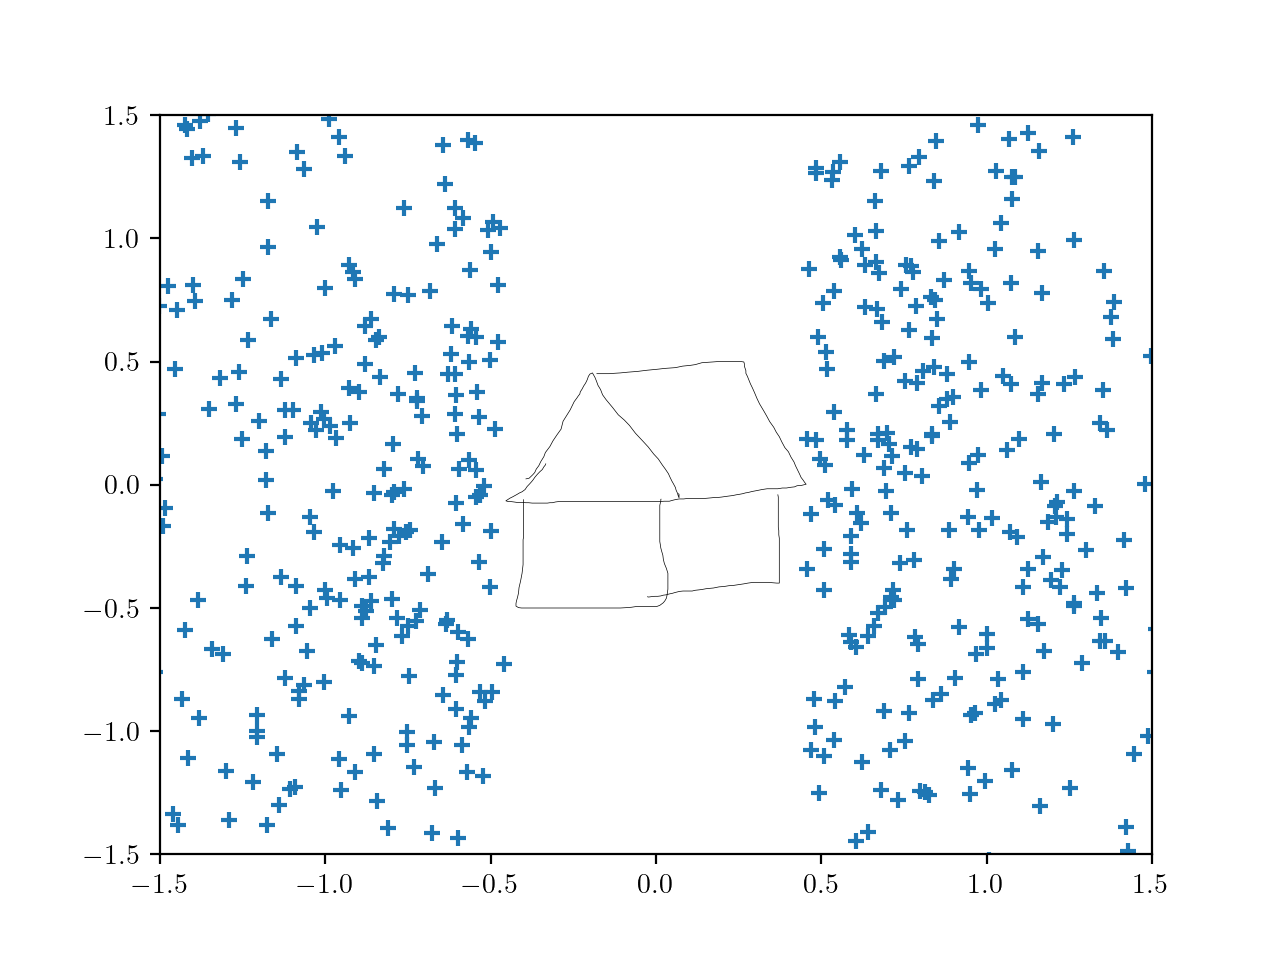
\includegraphics[width=\textwidth]{figures/rule_disjunct_side_house.png}
        \end{subfigure}
    \end{figure}
\end{frame}

\begin{frame}
    \frametitle{Rule-Based Approach}
    \begin{itemize}
        \item 5 handcrafted functions -- elementary constraints
        \begin{itemize}
            \item On Constraint
            \item Side Constraint
            \item Box Constraint
            \item Inside Constraint
            \item Disjunction Constraint
        \end{itemize}
        \item Constraint for each predicate is one or more combined elementary constraints.
    \end{itemize}
    \begin{figure}[ht]
        \centering
        \begin{subfigure}{0.45\textwidth}
            \centering
            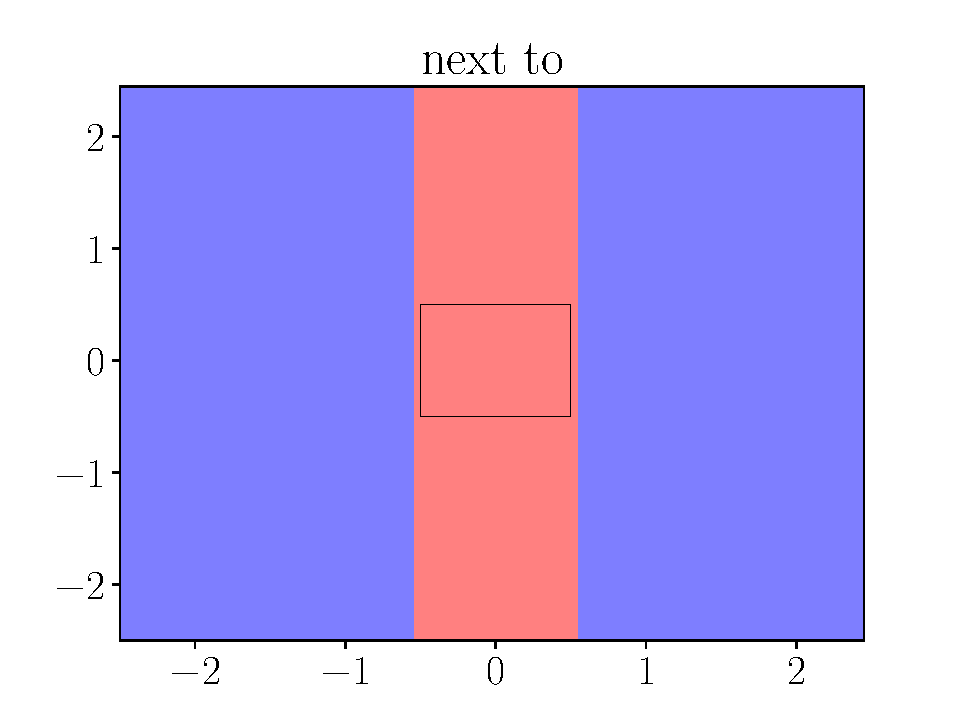
\includegraphics[width=\textwidth]{figures/next_to_rule}
        \end{subfigure}
        \begin{subfigure}{0.45\textwidth}
            \centering
            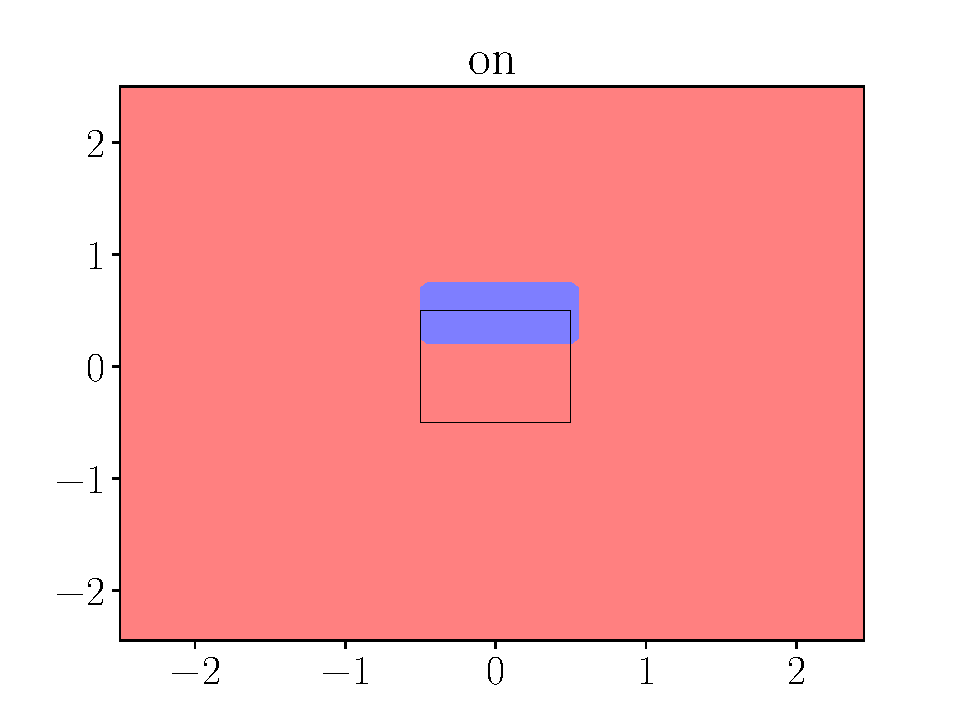
\includegraphics[width=\textwidth]{figures/on_rule}
        \end{subfigure}
    \end{figure}
\end{frame}

\begin{frame}
    \frametitle{First Classifier-Based Approach}
    \begin{itemize}
        \item A multilayer perceptron binary classifier trained on data from the \emph{Scene Graph} dataset.
        \item 52-dimensional input:
        \begin{itemize}
            \item 50-dimensional one-hot encoding of the semantic predicate;
            \item the last 2-dimensions represent the point in space (relative to the subject).
        \end{itemize}
    \end{itemize}
    \begin{figure}[ht]
        \centering
        \begin{subfigure}{0.45\textwidth}
            \centering
            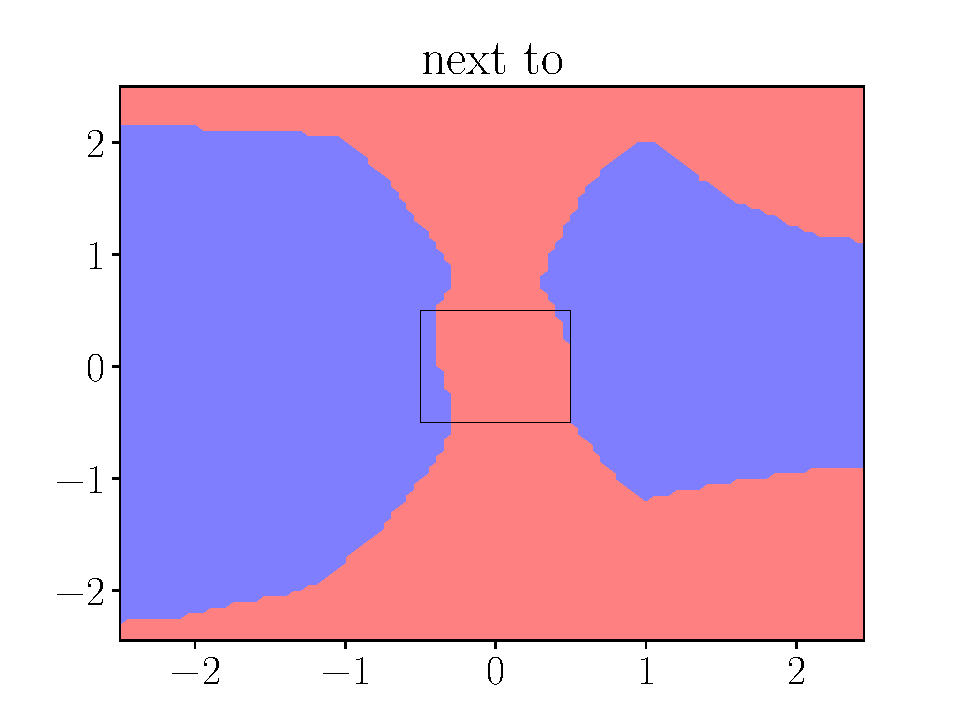
\includegraphics[width=\textwidth]{figures/next_to_predicate_only}
        \end{subfigure}
        \begin{subfigure}{0.45\textwidth}
            \centering
            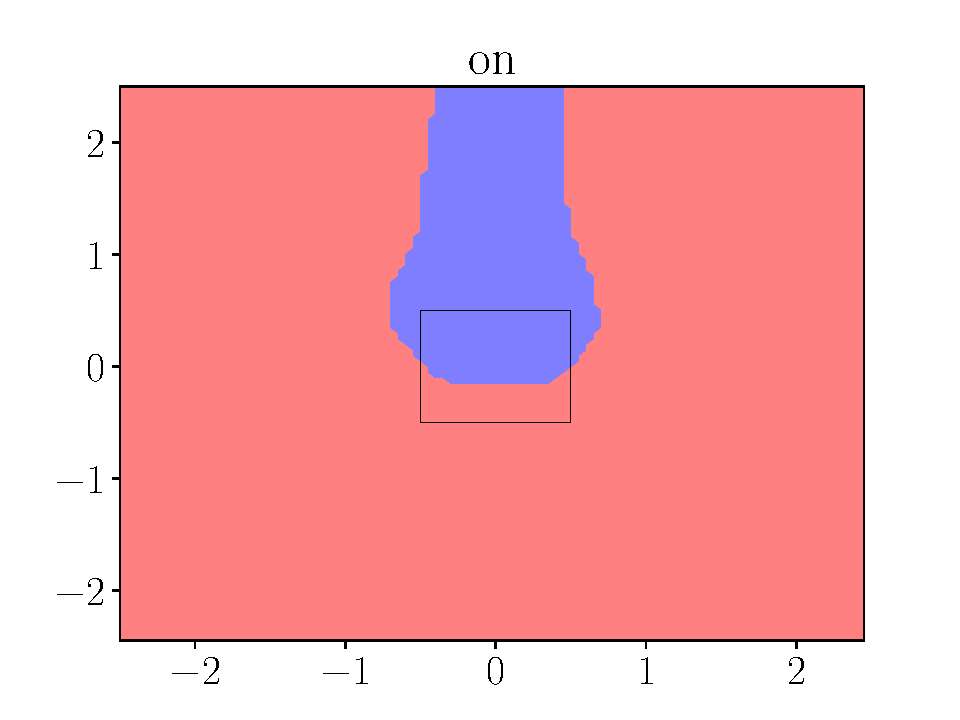
\includegraphics[width=\textwidth]{figures/on_predicate_only}
        \end{subfigure}
    \end{figure}
\end{frame}

\begin{frame}
    \frametitle{Comparing Rule-Based and Classifier-Based Constraints}
    \begin{figure}[ht]
    \centering
        \begin{subfigure}{0.45\textwidth}
            \centering
            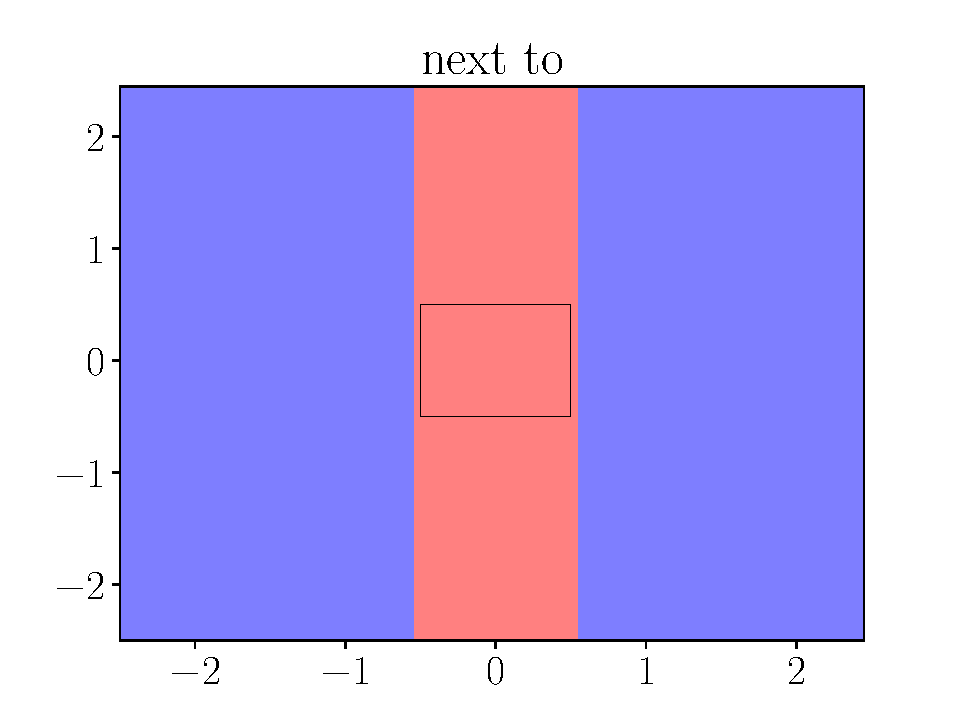
\includegraphics[width=\textwidth]{figures/next_to_rule.pdf}
        \end{subfigure}
        \begin{subfigure}{0.45\textwidth}
            \centering
            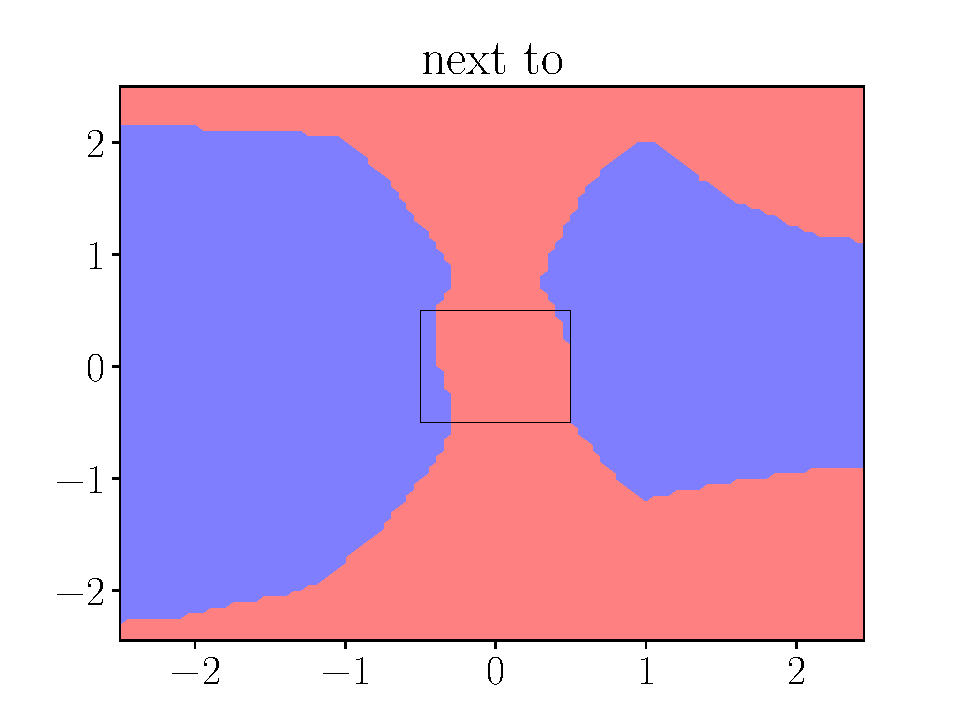
\includegraphics[width=\textwidth]{figures/next_to_predicate_only.pdf}
        \end{subfigure}
        \begin{subfigure}{0.45\textwidth}
            \centering
            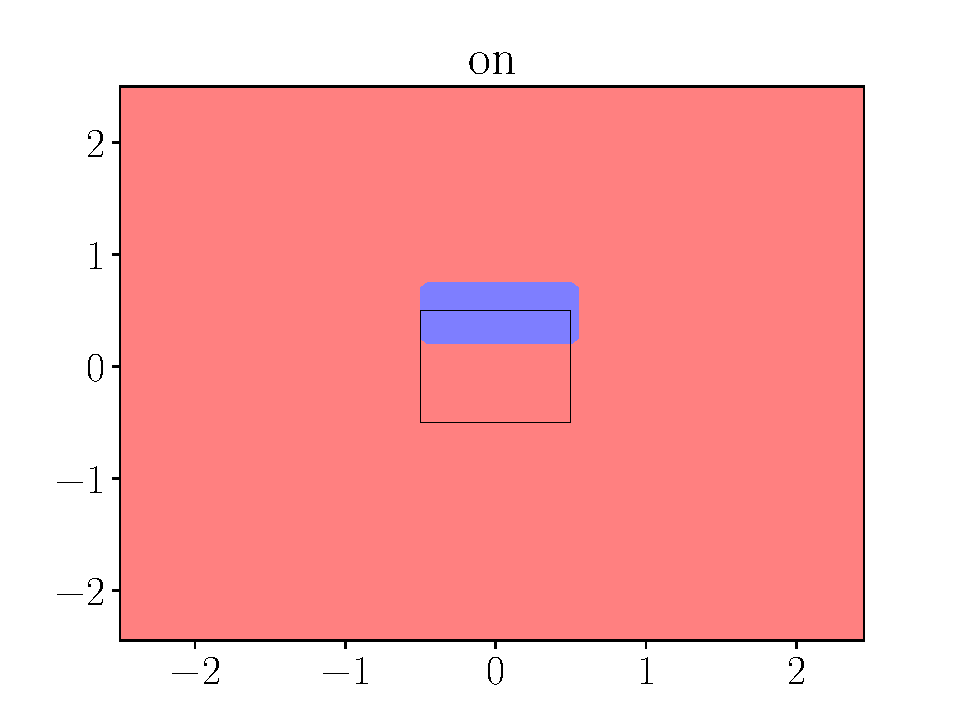
\includegraphics[width=\textwidth]{figures/on_rule.pdf}
        \end{subfigure}
        \begin{subfigure}{0.45\textwidth}
            \centering
            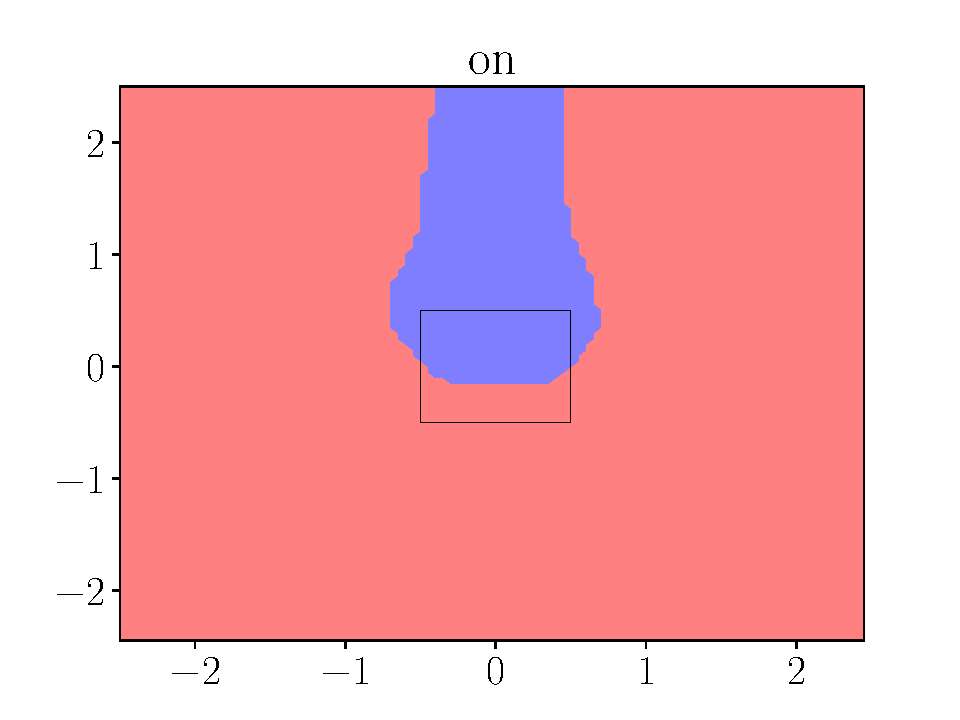
\includegraphics[width=\textwidth]{figures/on_predicate_only.pdf}
        \end{subfigure}
    \end{figure}
\end{frame}

\begin{frame}
    \frametitle{Comparing Rule-Based and Classifier-Based Constraints}
    \begin{figure}[ht]
        \begin{subfigure}{0.45\textwidth}
            \centering
            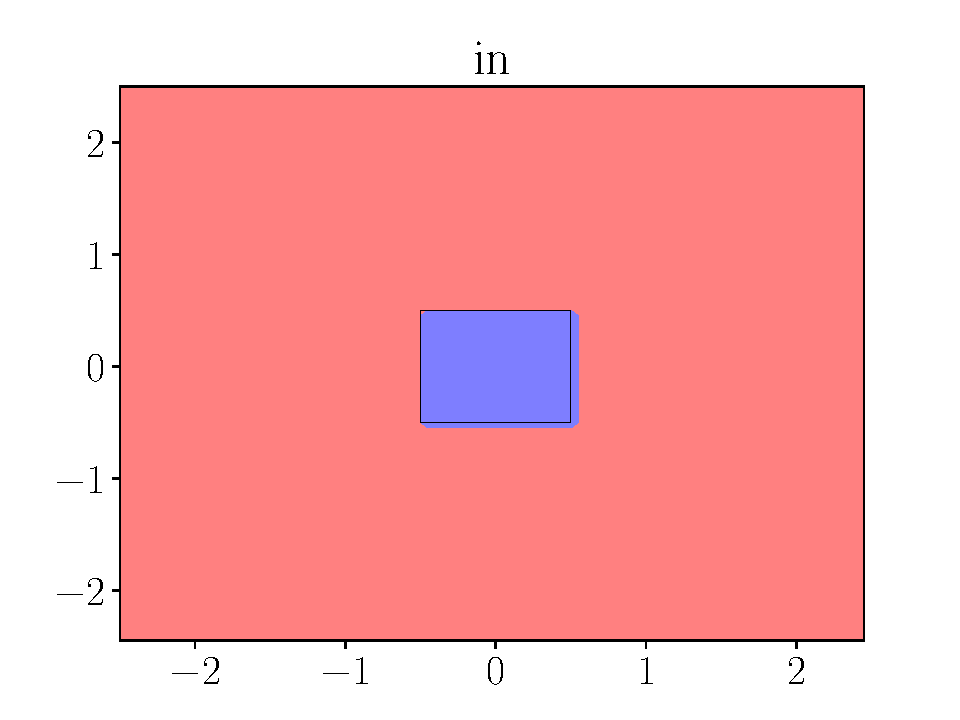
\includegraphics[width=\textwidth]{figures/in_rule.pdf}
        \end{subfigure}
        \begin{subfigure}{0.45\textwidth}
            \centering
            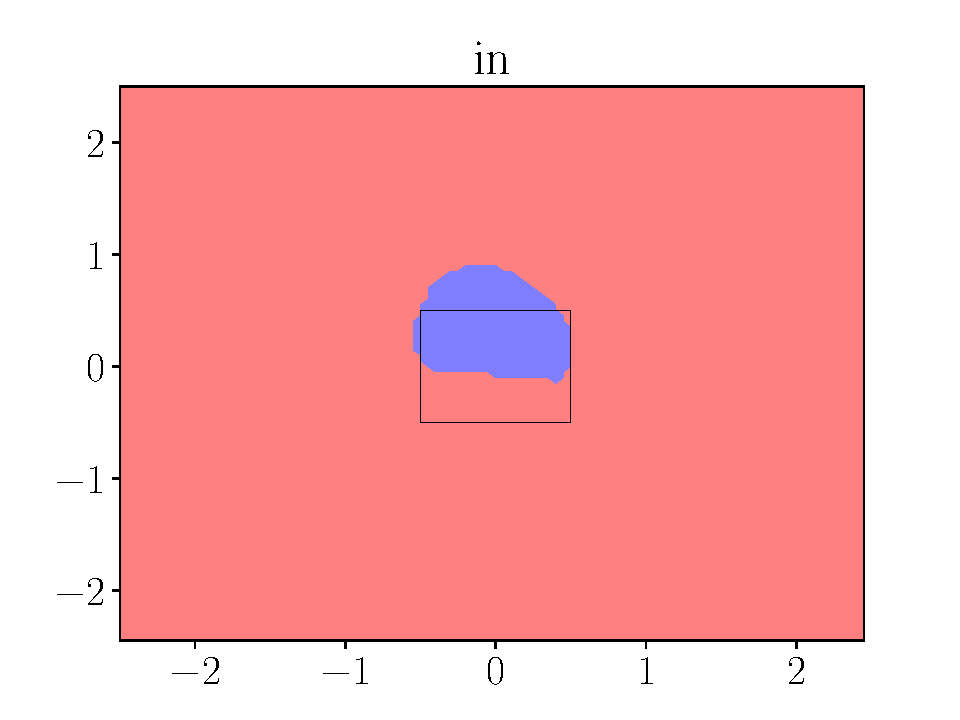
\includegraphics[width=\textwidth]{figures/in_predicate_only.pdf}
        \end{subfigure}
        \begin{subfigure}{0.45\textwidth}
            \centering
            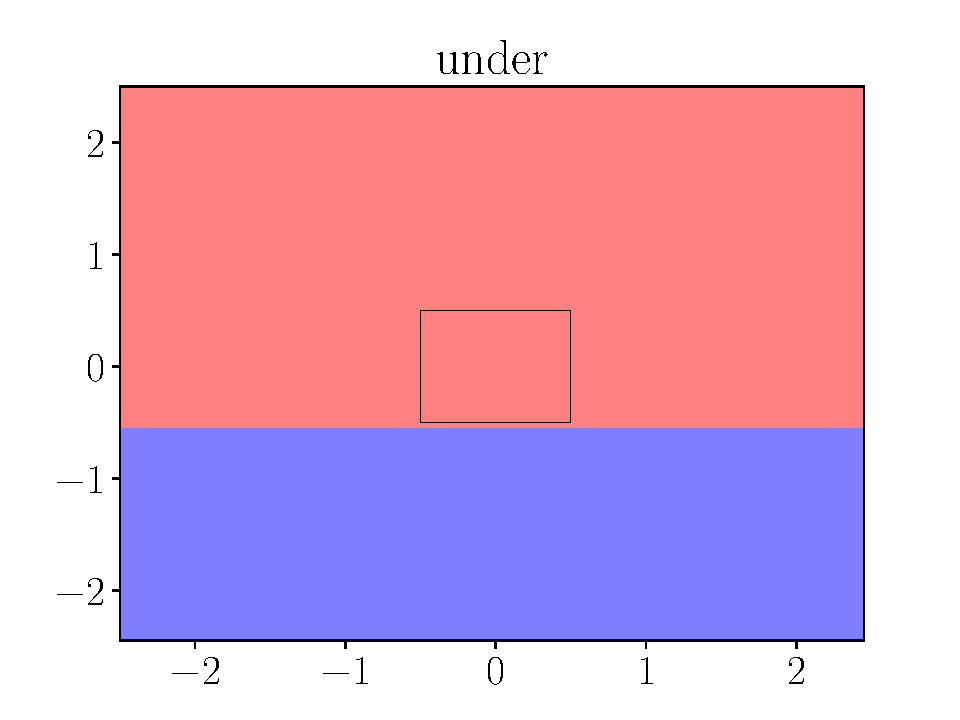
\includegraphics[width=\textwidth]{figures/under_rule.pdf}
        \end{subfigure}
        \begin{subfigure}{0.45\textwidth}
            \centering
            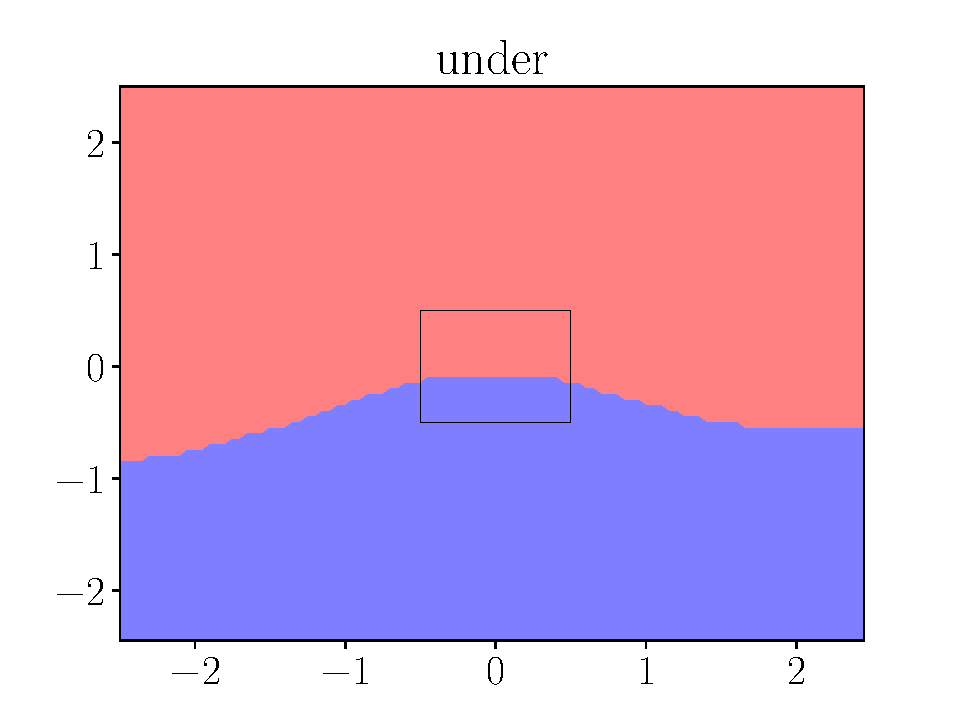
\includegraphics[width=\textwidth]{figures/under_predicate_only.pdf}
        \end{subfigure}
    \end{figure}
\end{frame}


\begin{frame}
    \frametitle{Second Classifier-Based Approach}
    \begin{itemize}
        \item Takes into account the object to which the constraint relates.
        \item 152-dimensional input:
        \begin{itemize}
            \item 100-dimensional word embedding of the semantic subject;
            \item 50-dimensional one-hot encoding of the semantic predicate;
            \item the last 2-dimensions represent the point in space (relative to the subject).
        \end{itemize}
    \end{itemize}
    \begin{figure}[ht]
        \centering
        \begin{subfigure}{0.45\textwidth}
            \centering
            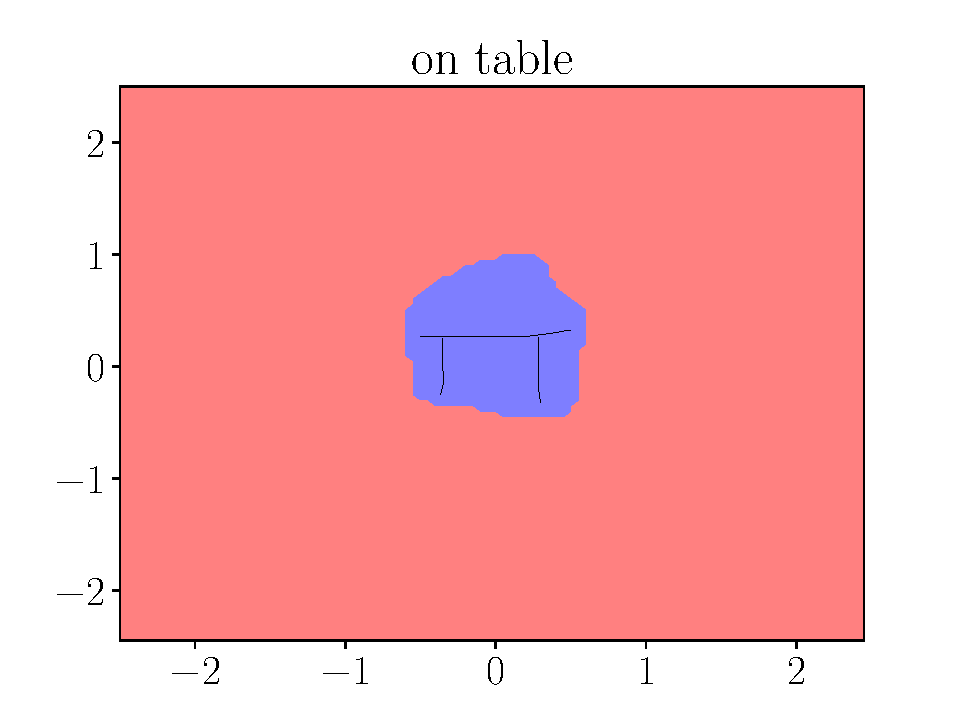
\includegraphics[width=\textwidth]{figures/on_table}
        \end{subfigure}
        \begin{subfigure}{0.45\textwidth}
            \centering
            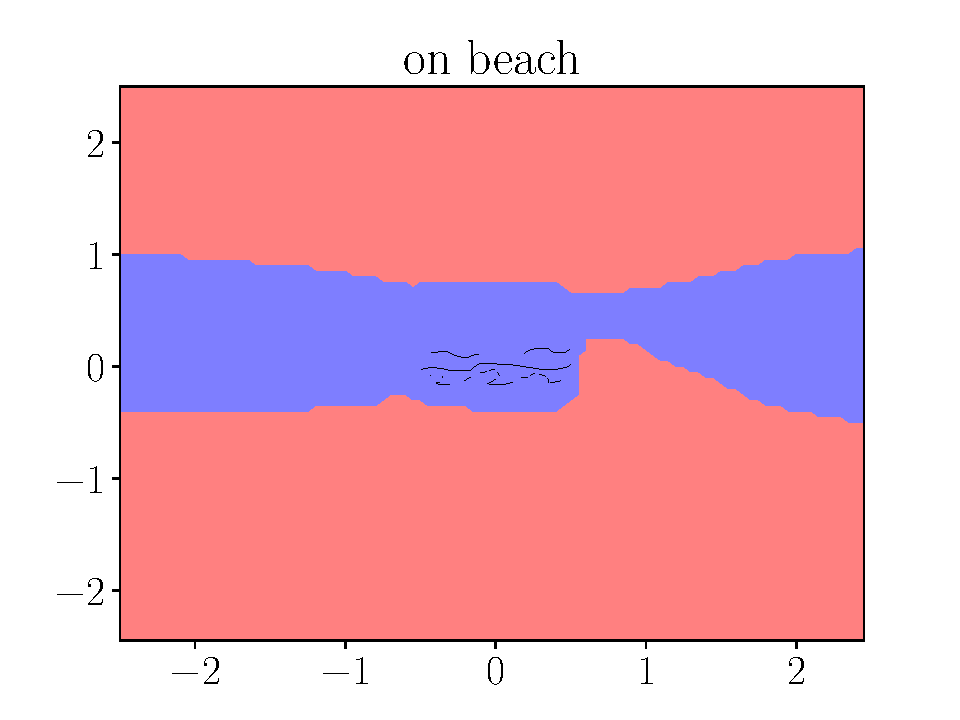
\includegraphics[width=\textwidth]{figures/on_beach}
        \end{subfigure}
    \end{figure}
\end{frame}

\begin{frame}
    \frametitle{Second Classifier-Based Approach Examples}
    \begin{figure}[ht]
    \centering
        \begin{subfigure}{0.45\textwidth}
            \centering
            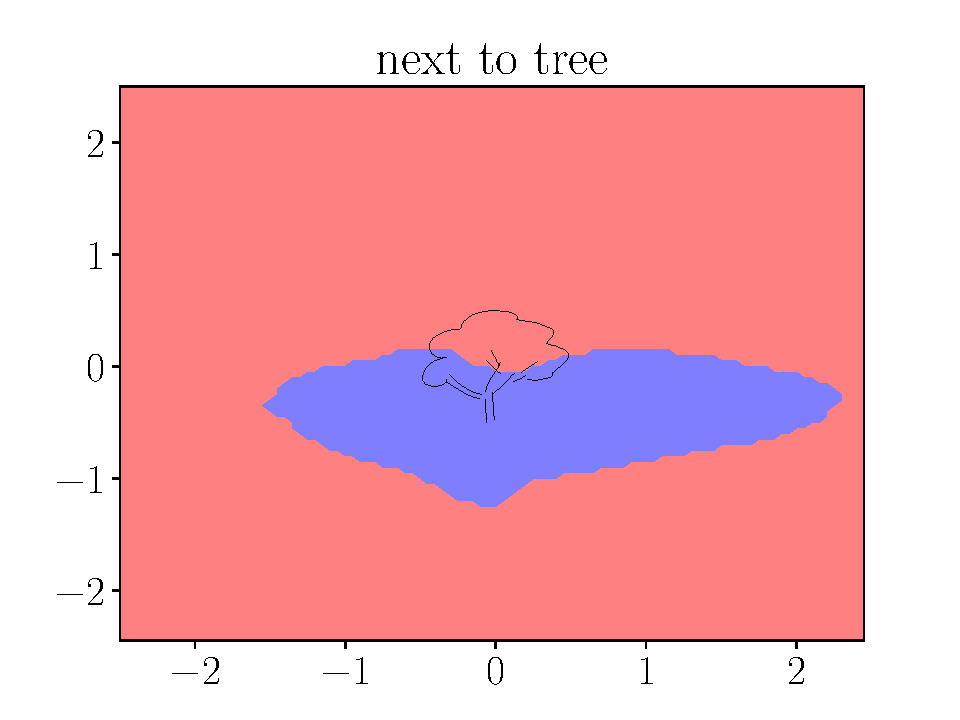
\includegraphics[width=\textwidth]{figures/next_to_tree.pdf}
        \end{subfigure}
        \begin{subfigure}{0.45\textwidth}
            \centering
            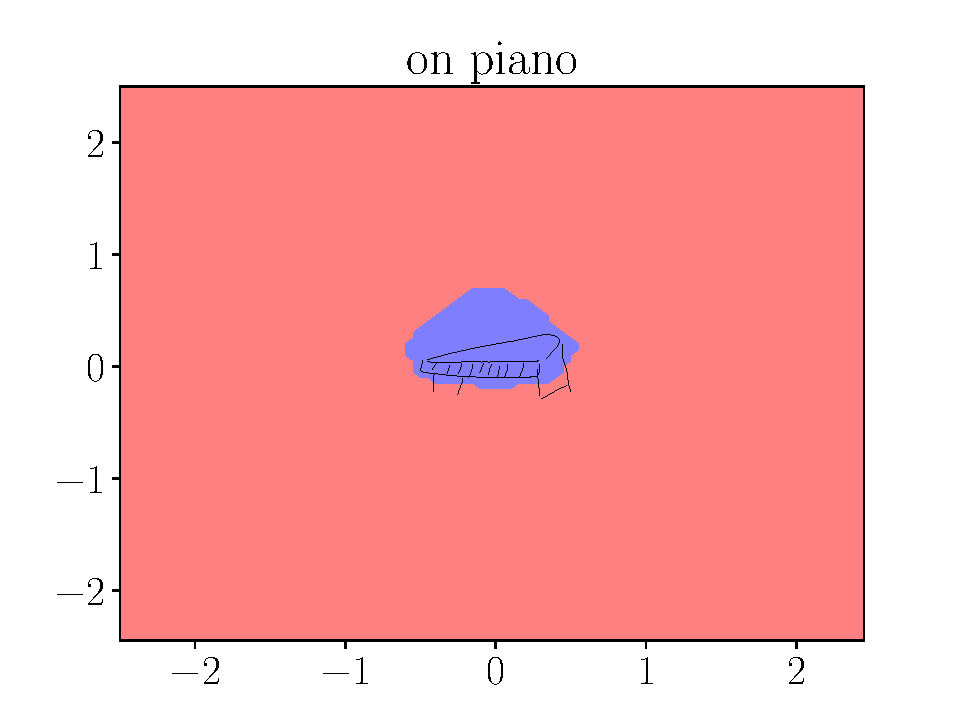
\includegraphics[width=\textwidth]{figures/on_piano.pdf}
        \end{subfigure}
        \begin{subfigure}{0.45\textwidth}
            \centering
            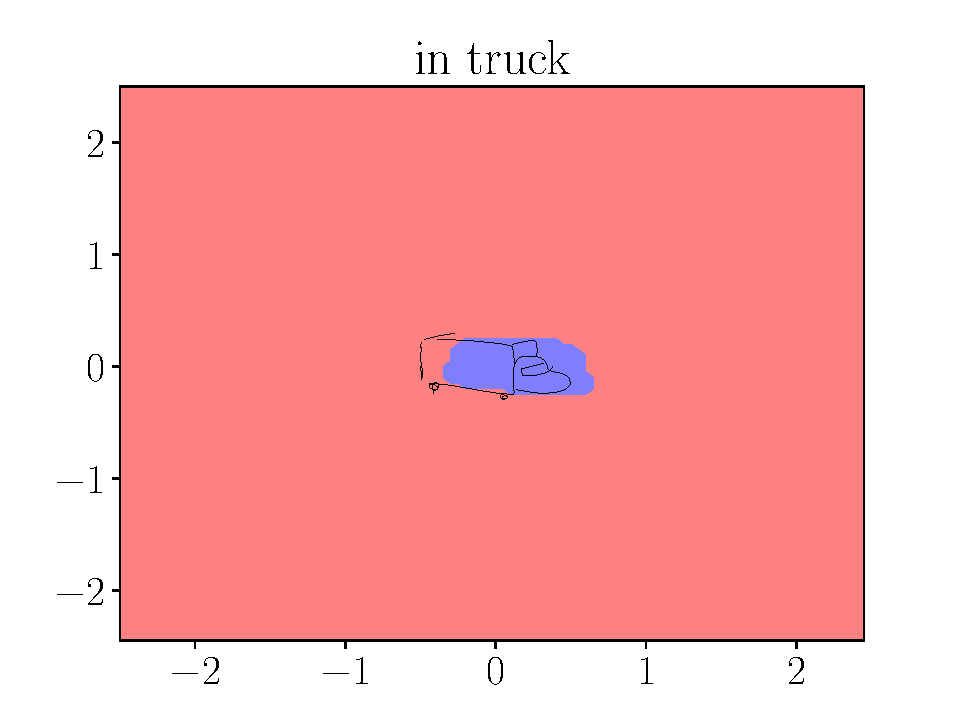
\includegraphics[width=\textwidth]{figures/in_truck.pdf}
        \end{subfigure}
        \begin{subfigure}{0.45\textwidth}
            \centering
            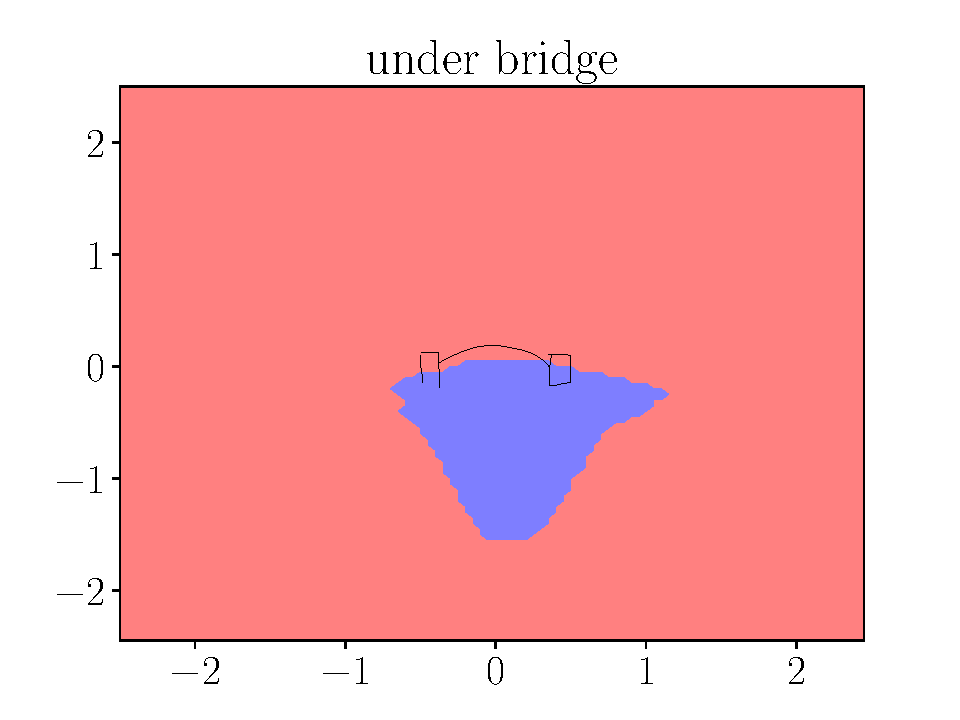
\includegraphics[width=\textwidth]{figures/under_bridge.pdf}
        \end{subfigure}
    \end{figure}
\end{frame}

\begin{frame}
    \frametitle{Determining Object's size}
    \begin{itemize}
        \item Absolute size approach:
        \begin{itemize}
            \item Manually estimated size for each object category.
            \item Automatic extraction from images is not feasible.
        \end{itemize}
        \item Relative size approach:
        \begin{itemize}
            \item Gathered automatically from the \emph{Scene Graph} dataset.
            \item Size ratio (ideally) for every pair of object categories.
            \begin{itemize}
                \item Not all pairs are covered by the dataset.
                \item Transitive closure.
                \item Similar words (word embedding cosine distance).
            \end{itemize}
        \end{itemize}
    \end{itemize}
    \begin{figure}[ht]
        \caption*{\say{A car is on the television.}}
        \centering
        \begin{subfigure}{0.35\textwidth}
            \centering
            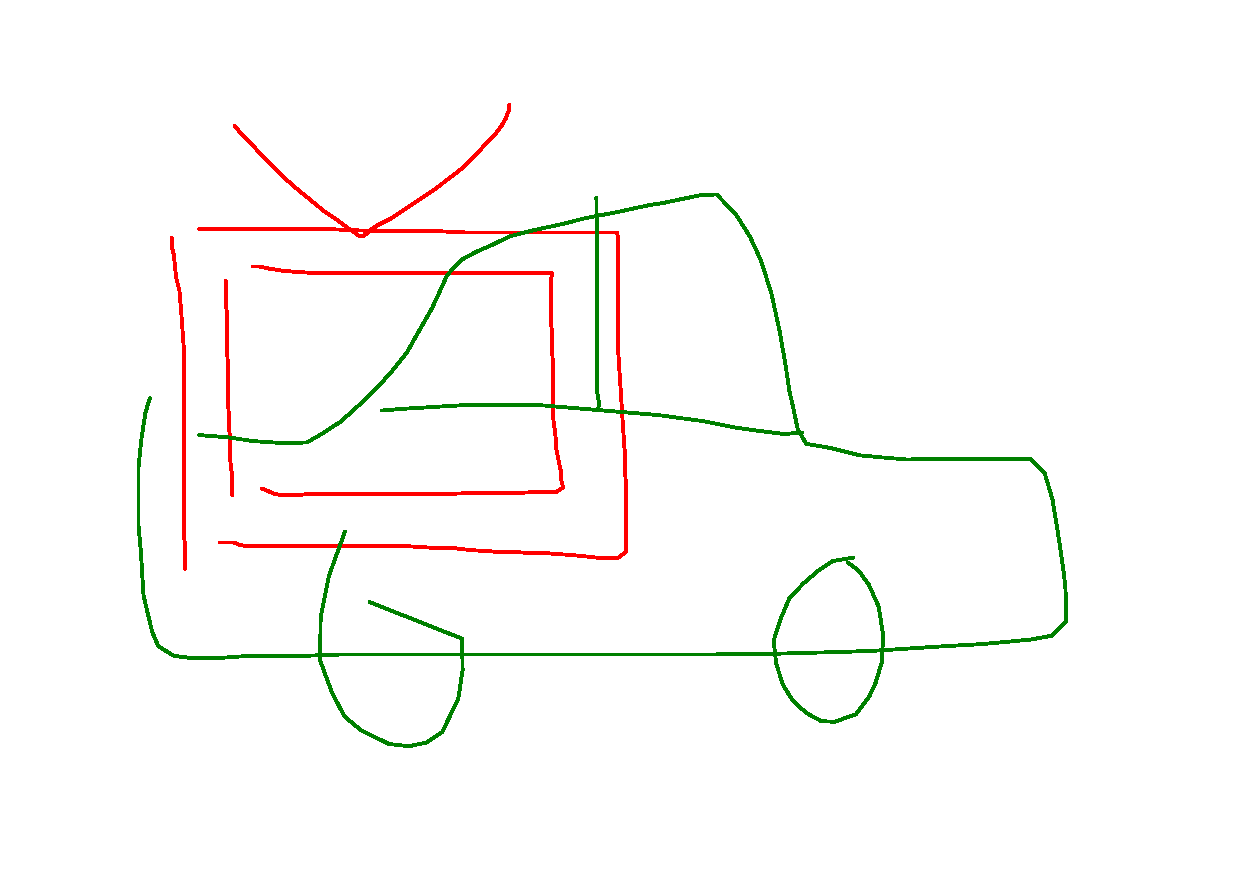
\includegraphics[width=\textwidth]{figures/car_on_tv_abs.pdf}
            \caption*{absolute size approach}
        \end{subfigure}
        \begin{subfigure}{0.35\textwidth}
            \centering
            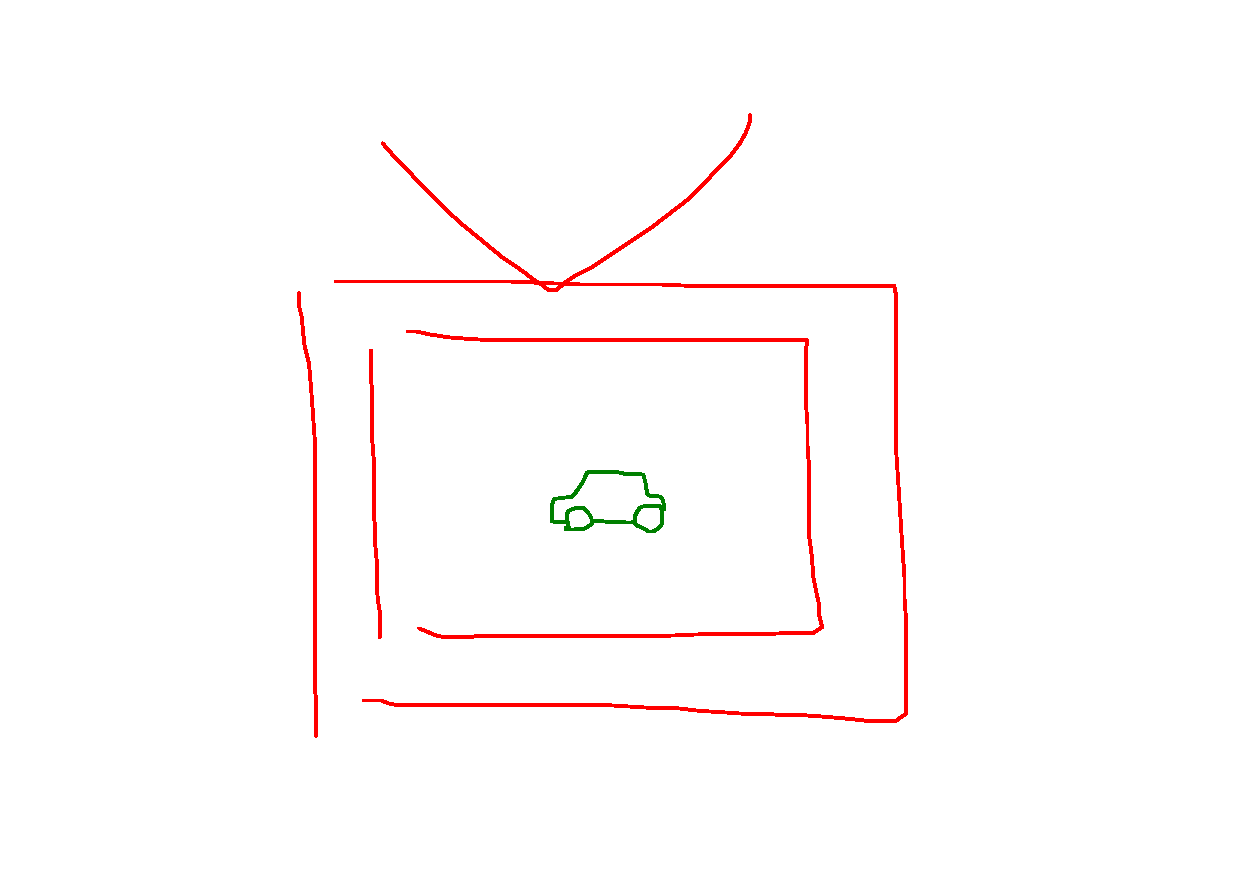
\includegraphics[width=\textwidth]{figures/car_on_tv_rel.pdf}
            \caption*{relative size approach}
        \end{subfigure}
    \end{figure}
\end{frame}

\begin{frame}[allowframebreaks,noframenumbering,plain]
    \frametitle{References}
    \bibliographystyle{plainnat} % Author (year)
    \bibliography{./bibliography}
\end{frame}

\end{document}
